\section{Combiner Ring}
\subsection{Injection}

\begin{figure}
\begin{center}
  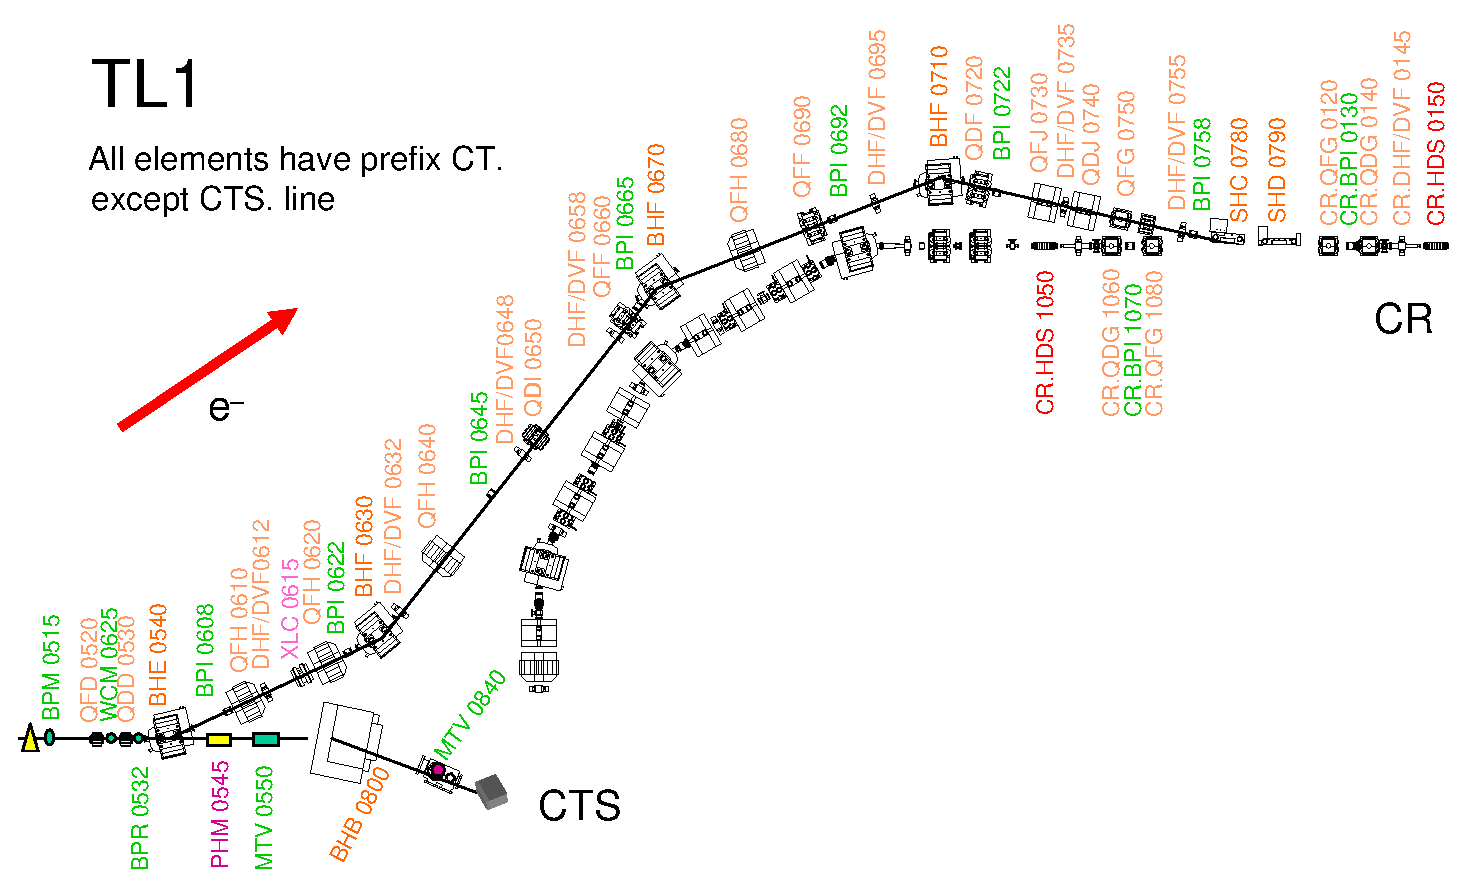
\includegraphics[width=0.96\linewidth]{tl1.eps}
  \caption{Annotated layout of the TL1 and injection region of the CR.}
\label{fig:tl1elements}
\end{center}
\end{figure}


Having beam fully setup in CTS, the next target was beam transport through
\ac{TL1}, injection to \ac{CR} and transport until the \ac{CRM} dump. 
During the initial setup the beam was inevitably entirely lost
therefore the shortest possible beam pulse was used, usually \textasciitilde 150~ns.
Figure~\ref{fig:tl1elements} shows the layout of this region.

Nominal optics was setup in the quadrupoles. 
Naturally, the initial bends and septa currents were setup using the theoretical excitation constants. 
They were tuned by switching off all the quadrupoles in \ac{TL1} line, adjusting the current 
of the first dipole family (CT.BHE0540-S), first to maximize 
the transported beam current over maximum number of BPMs, 
and in following to center the horizontal orbit over first two or three BPMs.
If the incoming orbit was well adjusted (and BPMs were well aligned) then it was possible to 
zero offsets on both CT.BPI0608 and CT.BPI0622. Otherwise the upstream corrector CT.BHB0510
together with CT.BHE0540-S were used to obtain this goal.
The quadrupoles in between bends CT.BHE0540 and CT.BHF0630 were switched on sequentially and 
change of orbit was recorded to asses eventual misalignments. 
If needed the orbit may was re-adapted using CT.BHF0540-S and CT.BHB0510. 
Afterwards the orbit correctors in between 
bends CT.BHE0540 and CT.BHF0630 were used to find lossless transmission over maximum
number of BPMs after CT.BHF0630 and to minimize the measured horizontal position.
This procedure was repeated until the beam reached the CR septa.


Initially, the magnetic injection was setup using steerer magnet CR.DHF0145 
(instead of the RF deflector) to bring the beam on the \ac{CR} orbit.
The main CR bend were left not powered to eventually direct the beam to the \ac{CRM} spectrometer line.
The quadrupoles were kept on and the septa current is adjusted to find
the horizontal beam position in CR.BPM0155 at -8~mm  when CR.DHF0145 was off.
This value corresponded to the model value in case the corrector magnet and the RF deflector were disabled.
Afterwards was CR.DHF0145 adjusted find the horizontal position readings at 
CR.BPM0155 and CR.BPM0195 as small as possible. At last, the corrector CR.DHF200 
was adapted to find the beam central on CRM.MTV0210.
 
In the next step dispersion was measured and if needed dispersion target steering was applied. 
In case correction with steerer magnets was not converging then quadrupoles would be used,
however, it was never necessary. In the next step the quality of the beam was verified with
a quad scan.

\subsection{RF Injection}

The setup of the inection with the RF deflector followed the logic described for the \ac{DL}.
%In order to setup the inection with the RF deflector \texttt{CR.HSD0150} 
The orbit for the magnetic injection was saved as a reference.
The aim was to setup the RF deflector to inject the beam on this reference and 
to assure that the RF phase corresponds to the crest of the RF wave.

The initial setting of the klystron power was first estimated using the measured RF amplitude.
The timing determining the end of the RF pulse was delayed to overlap with the beam pulse.
The phase was shifted such that beam was transported on the reference trajectory. 
This defined the first zero crossing phase. Naturally, it was expected that 
the second crossing was 180 degrees away and it was verified that was the case. 
If the discrepancy between the expected and the actual phase was large, above 10 degrees, 
then the calibration of the phase shifter was performed. 
If it was correct then the injecting phase (the crest) was defined as arithmetic average of 
the two zero crossing, i.e. in the perfect case 90 degrees away. 
With the RF deflector phase on the crest the orbit corrector CR.DHF0145-S was switched off.

In most cases the the amplitude of the RF deflector needed to be adjusted.
The procedure described above could have been iterated, however, 
it is quite lengthy in time because the klystron phase changes with the power level.
Therefore, the zero crossing phase needs to found at each step.

In CTF3 faster and more precise way was used. 
The procedure was repeated with two other power settings and for each of them 
the corresponding value of the phase knob was recorded. 
A linear fit was performed to the resulting power versus phase data points. 
The tangent coefficient gave number of degrees the phase need 
to be adjusted per power unit. Finally, the RF deflector power was adjusted and 
the phase was corrected using the matched coefficient. 
Eventually, the amplitude could be guessed in more systematic way. 
The orbit at the first BPM after the deflector was plotted versus
the power knob values and also fitted with a line. 
The obtained coefficients served to calculate the power corresponding 
to the reference orbit. However, the precision was good enough and
additional iterations were needed in most cases.

Finally, check if the phase corresponds to the \ac{CR}est was performed
by powering back corrector CR.DHF0145-S and moving the phase by 90 degrees.



\subsection{Setup of circulating beam}

The beam pulse length was adjusted to 200 - 280~ns. 
MKS21's end of RF timing was tuned to stop the RF deflector powering right 
after the last injected bunch. Because RF deflector filling time 
was very short (XX ns) 
\todo[inline]{Fill in the RF deflector filling time} 
such a pulse could circulate for thousands of turns.

After setting the nominal currents to the quadrupoles the bend circuit 
was adjusted to maximize the beam transmission and 
to minimize horizontal orbit around the ring, or 
at least over its initial part, if the beam was not losslessly transported 
over the full turn. Eventually, some manual obit correction was done to thread 
the beam over the first turn.
Afterwards, automatic one-to-one orbit correction was performed followed by
automatic closure. In most cases it permitted to have the beam circulating over 
circa 10 turns. 

As the last step the dispersion was verified and eventually corrected using 
Dispersion Target Steering followed by the orbit closure.

\subsection{Ring Length}

The orbit length had to be precisely $N+\frac{1}{4}\times \lambda_{RFD}$, 
where $N$ is is an integer number (848 according to the design) and 
$\lambda_{RFD}$ was wavelength of the RF deflector (2.998~GHz).
This was required for the beam recombination process. The most precise way to measure 
the ring length, and to adjust the wigglers, was based on FFT of the beam phase signal
measured with CR.BPR0505 for the circulating beam which is detailed in Section~\ref{sec:ringlen}.


\subsection{RF bump}

As the first step the orbit of the circulating beam was saved as a reference.
On the second turn the beam should pass the deflectors on zero crossing phase.
On the third one on maximum amplitude opposite to the injection one. The fourth turn
should correspond to the second zero crossing. 
Mechanical attenuator of the second RF deflector CR.HDS1050 was set to
to stop all the RF power. MKS21 RF pulse was made 280 longer 
%using CX.MKS21ERF \todo{check name of end of RF for 21}) knob 
so it was powered during the second beam pulse passage through CR.HDS0150.
If the orbit of the second turn changed it meant that the ring length was not right
and the wigglers needed to be tuned. Afterwards, RF pulse for the RF deflectors was made
another 280~ns longer to cover the $3^{rd}$ turn. 
Attenuator of the 2nd deflector changed to deliver the power. 
Phase had to be first adjusted to make the 2nd turn orbit stay on reference.

If the 3rd turn was not closed the attenuator had to be adjusted to adapt the kick amplitude 
of the 2nd RFD, at each step adjusting the phase to keep the 2nd turn orbit on the reference.
When completed, the RF pulse was elongated by another 280~ns to cover the 4th turn
and normally the orbit should bot change. Usually a further small adjustment on phase and 
power of the 2nd RFD was needed. 

At this point lengthening the beam pulse to 1120~ns made a factor four recombined beam.


\subsection{Orbit through RF deflectors}

The procedure above would complete the setup in case of the perfect alignment.
In reality, in CTF3 the RF deflectors were offset with respect of the orbit 
defined by the BPMs. Alignment of CTF3 was rather poor, however, 
in the latter case the situation was particularly 
difficult because these deflectors were not equipped with 
the CERN standard fiducialization targets. 
Therefore, non standard less precise procedure was applied.

In case the beam passed the RF deflectors off their axis it induced longitudinal wake,
which had several implications. First, if cavity was not powered bunch would lose its energy 
on every passage.
\todo[inline]{Any transverse kick for $\lambda/4$ delayed beam.?}
If the cavity was powered the bunches would be accelerated or decelerated depending on
the respective phase. 

In order to minimize the effect the orbit was adjusted to minimize loading effect of each deflector
which was clearly visible at the RF power measured at the output couplers of the deflectors.
Septa and correctors in \ac{TL1} were used to change the orbit until the beam effect was not visible on 
the measured trace.
Alternatively, a closed bump calculated with the model was used. 


\subsection{Ejection}

The layout of the ejection was the same as of the injection, 
but of course a kicker magnet replaced an RF deflector.
A great nuisance was the common powering of injection and ejection septa.
Given the far from ideal alignment and limitted number of the orbit correctors
it was quite difficult to adjust the orbit such that 
the beam cleanly passed the long straight section while circulating in the ring
and be well ejected into the TL2. 
In such occation the septa powering was eventually corrected and
the injection orbit, dispersion and the orbit closure in the ring had to be reworked.

















